
Методы решения задач компьютерного зрения могут основываться как классических подходах, так и на применении глубоких нейронных сетей.

Классические методы построены на анализе внутренней структуры и симметрии изображения, его семантике и характеристиках объектов на нем. 
Эти методы включают в себя алгоритмы обработки изображений, фильтрацию, выделение признаков (например, метод гистограмм градиентов или методы локтевых точек),
шаблонное сопоставление и классификацию на основе характеристик объектов.

\textit{Определение:}\textbf{Сверточные нейронные сети} (CNN)\cite{lecun1989handwritten} представляют собой класс глубоких нейронных сетей,
использующих специально разработанные для обработки структурно-связанных данных как изображения. 

Эффективность CNN определяется их возможностью  извлекать иерархические признаки из входных данных.

\begin{figure}[h]
    \centering
    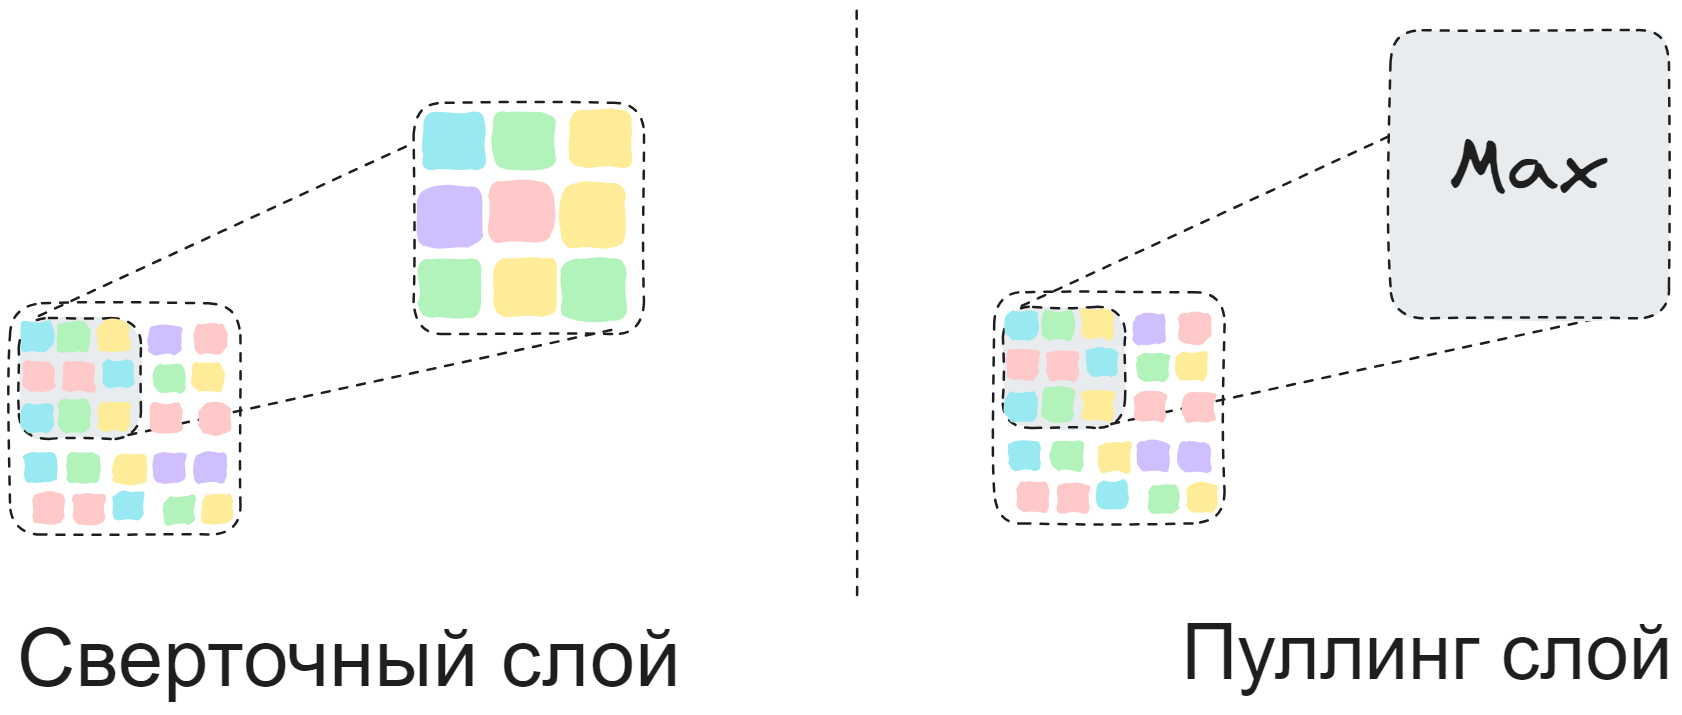
\includegraphics[width=0.5\textwidth]{assets/ml/cv/conv.excalidraw.png}
    \caption{Сверточный слой содержит параметрическое ядро, обеспечивающее выделение ключевых признаков. Пуллинг-слои выполняют заранее заданную аналитическую операцию.}
    \label{cnn}
\end{figure}

Глубокие методы, основанные на сверточных нейронных сетях (CNN), 
стали широко распространенными и эффективными в решении задач компьютерного зрения. 
Эти методы автоматически изучают признаки изображений на различных уровнях абстракции, 
начиная от низкоуровневых признаков, таких как грани и текстуры, до высокоуровневых семантических признаков,
связанных с объектами и их распознаванием. 
 
Основными компонентами сверточных нейронных сетей являются:
 \begin{itemize}
    \item сверточные слои --- выполняют операции свертки над входными данными с использованием фильтров или ядер, 
    чтобы извлечь локальные пространственные признаки, такие как грани, углы и текстуры, что позволяет модели обнаруживать 
    абстрактные особенности изображений на разных уровнях детализации;
    \item пуллинг-слои --- предназначены для уменьшения пространственных размеров активаций, полученных после сверточных операций, путем 
    объединения пикселей в заданных областях, что позволяет модели быть устойчивой к небольшим искажениям объектов 
    на изображении и уменьшает количество параметров,  снижает переобучение и способствует росту эффективности вычислений;
    \item полносвязанные слои обычно располагаются в конце архитектуры нейронной сети и используются для объединения высокоуровневых признаков, 
    извлеченных предыдущими слоями, в предсказаниях или классификации.
\end{itemize}
 
Во время обучения сверточной нейронной сети параметры каждого слоя оптимизируются с использованием специальных методов, таких как обратное 
распространение ошибки и стохастический градиентный спуск. Целью является минимизация заданной функции потерь. Этот процесс позволяет настраивать 
параметры модели для эффективного извлечения признаков и выполнения конкретной задачи, такой как классификация изображений или сегментация объектов.

\begin{figure}[h]
    \centering
    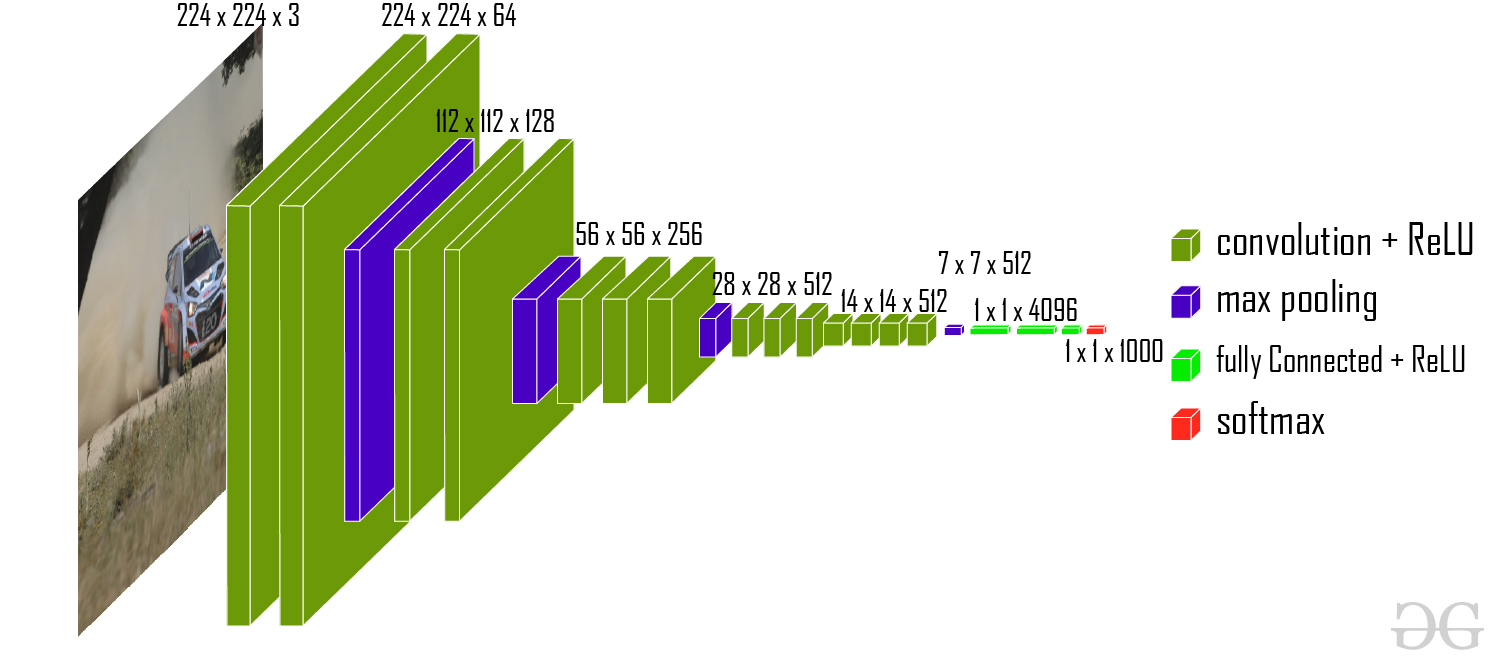
\includegraphics[width=0.5\textwidth]{assets/ml/cv/vgg16.jpg}
    \caption{Архитектура VGG16 \cite{simonyan2014very}}
    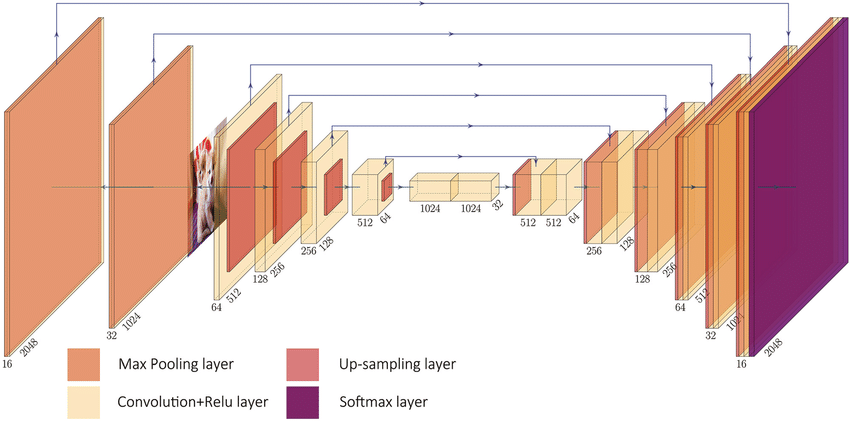
\includegraphics[width=0.5\textwidth]{assets/ml/cv/unet.png}
    \caption{Архитектура Unet \cite{ronneberger2015u}.}
    \label{vgg_arch}
\end{figure}

Архитектуры U-Net и ResNet \ref{vgg_arch} привнесли существенные модификации в оригинальные архитектуры сверточных сетей 
\begin{itemize}
    \item использование симметричной структуры, деконволюционные слои (upsampling) для восстановления пространственного разрешения;
    \item блоки с пропуском, обеспечивающие плавное обучение глубоких сетей  $x_{t+1} = x_t + \phi_t(x_t)$, где $\phi_t(x)$ --- функция активация промежуточного слоя $t$.
\end{itemize}

Методы аугментации изображений в компьютерном зрении представляют собой техники, используемые для увеличения размера и разнообразия тренировочного набора данных путем
применения различных преобразований к изображениям. Целью аугментации является создание дополнительных вариаций изображений, что помогает улучшить обобщающую способность
моделей машинного обучения и снизить риск переобучения.

Основные методы аугментации включают в себя:
\begin{itemize}
    \item изменение размера изображения (путем масштабирования);
    \item поворот и отражение; 
    \item изменение яркости, контраста и насыщенности цветов;
    \item добавление шума или размытия.
\end{itemize}    
    
Дополнительно могут применяться специфические трансформации, такие как сдвиги, обрезка или изменение геометрии изображения.

Применение методов аугментации позволяет модели обучаться получать на более разнообразных данных, 
что способствует повышению устойчивости модели в различных условиях. Кроме того, аугментация позволяет уменьшить влияние 
несбалансированности классов и улучшить обобщающую способность моделей.

Модель YOLO (You Only Look Once) представляет собой популярную архитектуру для обнаружения объектов на изображениях. 
Основной идеей является выполнение обнаружения объектов и их классификации в одной сети, что делает ее быстрой и эффективной \cite{kirillov2023segment}.

Порядок работы модели YOLO начинается с входного изображения, которое подается на вход нейронной сети. Затем изображение проходит через сверточные слои, которые извлекают 
из изображения признаки на различных уровнях абстракции. Далее, полученные признаки проходят через сверточные слои, которые прогнозируют ограничивающие рамки (boxes) для объектов 
и вероятности их принадлежности к различным классам. Эти сверточные слои выполняют прогнозы на основе якорей (anchors), которые представляют разные размеры и соотношения 
сторон ограничивающих рамок. После этого выполняется пост-обработка, включающая подавление неоднородных предсказаний (non-maximum suppression), чтобы получить итоговые прогнозы объектов. 
Этот шаг удаляет дубликаты и прогнозирует объекты с наибольшей уверенностью (confidence).

Результатом работы модели YOLO является набор ограничивающих рамок с идентификацией классов объектов, найденных на изображении и оценками уверенности. 
Модель обеспечивает возможность работы в масштабе времени близком к реальному.


Для любых матриц $A$ и $B$ выполняется:
\begin{equation}
    \text{rang}(AB) \le \min\left(\text{rang}(A),\text{rang}(B)\right)
\end{equation}
   
Низкоранговый адаптер Lora работает путем сжатия параметров модели с использованием низкоранговых матриц. Основная идея заключается в том, 
чтобы аппроксимировать исходные параметры модели с помощью матриц меньшего ранга. Это позволяет снизить объем памяти,необходимый для хранения 
параметров и ускорить вычисления.
\begin{figure}[h]
    \centering
    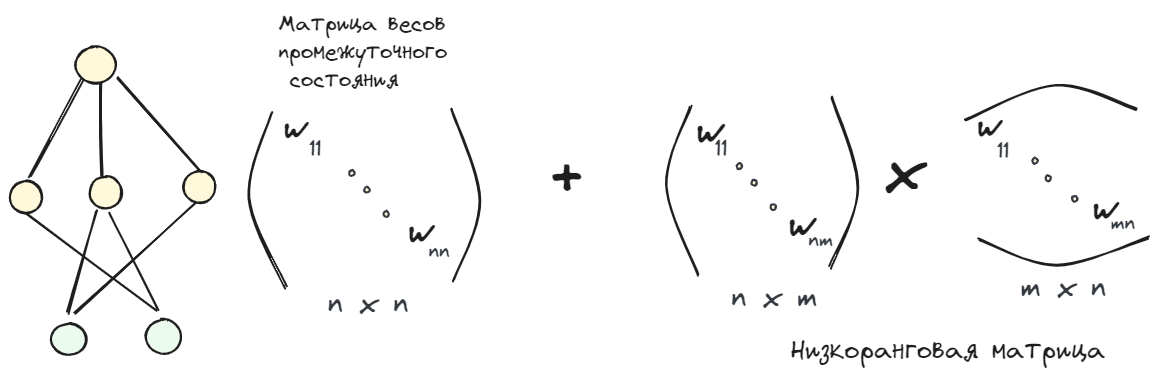
\includegraphics[width=0.5\textwidth]{assets/ml/adapter/adapter.excalidraw.png}
    \caption{Модель адаптера \text{Lora} \cite{hu2021lora}}
    \label{sd_learning}
\end{figure}

Наиболее популярным вариантом адаптера является Lora \cite{hu2021lora}:
\begin{equation}
    \hat{W} = W + AB,
\end{equation}
где  $AB$ --- низкоранговая матрица, полученная произведением матриц $A$ размерности \( m \times r \) и  $B$ размерности  $r \times n$,
где \( r \) --- это ранг аппроксимации.
